\documentclass[24pt]{beamer}
\usepackage[utf8]{inputenc}
\usepackage[utf8]{vietnam}
\usepackage{amsmath}
\usepackage{amsfonts}
\usepackage{amssymb}
\usepackage{graphicx}
\usepackage{tikz}
\usetikzlibrary{positioning}
\usepackage{xcolor}
\usepackage{utopia}
\usepackage{siunitx}
\usepackage[american,cuteinductors,smartlabels]{circuitikz}
\usepackage{ragged2e}
\usepackage{etoolbox}

\usepackage{enumerate}
\mode<beamer>{\usetheme{CambridgeUS}}

\usecolortheme{default}

\usepackage{hyperref}
\hypersetup{pdfpagemode=FullScreen} %mode FullScreen with beamer

\apptocmd{\frame}{}{\justifying}{} % Allow optional arguments after frame.

\usepackage{comment}

\makeatletter
\let\insertuniversity\relax
\newcommand\universitytitle{TRƯỜNG ĐH}

\let\insertclass\relax
\newcommand\classtitle{Lớp}

\let\insertcourse\relax
\newcommand\coursetitle{Môn học}

\mode<all>
{
  \newcommand\university[1]{\def\insertuniversity{#1}}
  
  \newcommand\class[1]{\def\insertclass{#1}}
  
  \newcommand\course[1]{\def\insertcourse{#1}}
  \titlegraphic{}
}

\defbeamertemplate*{title page}{supdefault}[1][]
{
  \begingroup
    \centering
    \ifx\insertuniversity\relax\relax\else
    \begin{beamercolorbox}[sep=2pt,center,#1]{author}
      \hspace{-.15cm}\scriptsize\universitytitle~\insertuniversity
    \end{beamercolorbox}\fi

    \vspace{-.1cm}
    \begin{beamercolorbox}[sep=8pt,center,#1]{title}
      \usebeamerfont{title}\normalsize\inserttitle\par%
      \ifx\insertsubtitle\@empty\relax%
      \else%
        \vskip0.25em%
        {\usebeamerfont{subtitle}\usebeamercolor[fg]{subtitle}\insertsubtitle\par}%
      \fi%     
    \end{beamercolorbox}%
    \vskip.5em\par

    \vspace{-.4cm}
    \ifx\insertcourse\relax\relax\else
    \begin{beamercolorbox}[sep=6pt,center,#1]{author}
      \usebeamerfont{author}\footnotesize\coursetitle:~\insertcourse
    \end{beamercolorbox}\fi

    \vspace{-.3cm}
    \ifx\insertclass\relax\relax\else
    \begin{beamercolorbox}[sep=6pt,center,#1]{author}
      \usebeamerfont{author}\footnotesize\classtitle:~\insertclass
    \end{beamercolorbox}\fi

    \vspace{-.3cm}
    \begin{beamercolorbox}[sep=6pt,center,#1]{author}
      \usebeamerfont{author}\hspace{-.23cm}\footnotesize\insertauthor
    \end{beamercolorbox}
    %\begin{beamercolorbox}[sep=8pt,center,#1]{institute}
      %\usebeamerfont{institute}\insertinstitute
    %\end{beamercolorbox}
    \vspace{-.4cm}
    \begin{beamercolorbox}[sep=8pt,center,#1]{date}
      \usebeamerfont{date}\footnotesize\insertdate
    \end{beamercolorbox}\vskip0.5em
    {\usebeamercolor[fg]{titlegraphic}\inserttitlegraphic\par}
  \endgroup
  \vfill
}
\setbeamertemplate{title page}[supdefault][colsep=-4bp,rounded=true,shadow=\beamer@themerounded@shadow]\makeatother

%Title page
\title[KT Lập trình tuần tự]{\emph{Chủ đề báo cáo}\\ Ứng dụng KT lập trình tuần tự vào TK hệ thống điều khiển}
\author[TK Hệ thống điều khiển]{GVHD: Nguyễn Khắc Nguyên \and SVTH: N4}
\course{Thiết kế hệ thống điều khiển}
\class{Công nghệ, kỹ thuật điện, điện tử}
\university{KỸ THUẬT -- CÔNG NGHỆ CẦN THƠ}
\date[Nhóm 4]{Thời gian: \today}

\AtBeginSection[]
{
  \begin{frame}
    \frametitle{Nội dung báo cáo}
    \justifying
    \tableofcontents[currentsection]
  \end{frame}
}
\definecolor{doden}{RGB}{204, 0, 0}
\newcommand{\noibat}[1]{\textcolor{blue}{#1}}
\begin{document}
%http://tex.stackexchange.com/questions/82794/removing-page-number-from-title-frame-without-changing-the-theme
\bgroup
\makeatletter
\setbeamertemplate{footline}
{
  \leavevmode%
  \hbox{%
  \begin{beamercolorbox}[wd=.333333\paperwidth,ht=2.25ex,dp=1ex,center]{author in head/foot}%
    \usebeamerfont{author in head/foot}\insertshortauthor\expandafter\beamer@ifempty\expandafter{\beamer@shortinstitute}{}{~~(\insertshortinstitute)}
  \end{beamercolorbox}%
  \begin{beamercolorbox}[wd=.333333\paperwidth,ht=2.25ex,dp=1ex,center]{title in head/foot}%
    \usebeamerfont{title in head/foot}\insertshorttitle
  \end{beamercolorbox}%
  \begin{beamercolorbox}[wd=.333333\paperwidth,ht=2.25ex,dp=1ex,right]{date in head/foot}%
    \usebeamerfont{date in head/foot}\insertshortdate{}\hspace*{2em}
%    \insertframenumber{} / \inserttotalframenumber\hspace*{2ex}
    \hspace*{6ex}
  \end{beamercolorbox}}%
  \vskip0pt%
}

\begin{frame}
\titlepage
\end{frame}
\egroup

\setcounter{framenumber}{0}

%--------------------------------------------------------------------------------
%--------------------------------------------------------------------------------
% Danh sach thanh vien
\begin{frame}{Danh sách thành viên}
	\vspace{-.5cm}
	\begin{small}
	\begin{columns}
		\column{0.6\textwidth}
		\begin{enumerate}
			\item Nguyễn Văn Đình
			\item Thi Minh Nhựt
			\item Phạm Thanh Quý
			\item Hồ Minh Thành
			\item Liên Thái Trường
			\item Lư Anh Tuấn
			\end{enumerate}

		\column{.4\textwidth}
		\begin{enumerate}
			\item[] 1350353
			\item[] 1350366
			\item[] 1350222
			\item[] 1350444
			\item[] 1350358
			\item[] 1350240
		\end{enumerate}
	\end{columns}
		\end{small}
\end{frame}

%--------------------------------------------------------------------------------
%--------------------------------------------------------------------------------
% Noi dung bao cao
\begin{frame}
	\frametitle{Nội dung báo cáo}
	\tableofcontents
\end{frame}
%--------------------------------------------------------------------------------
%--------------------------------------------------------------------------------
\section{Chủ đề báo cáo}
\begin{frame}{Đề bài -- Bài tập 4}
	\vspace{-.5cm}
	\hspace{-1cm}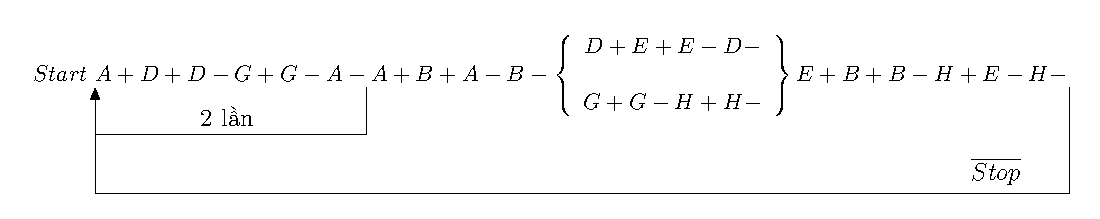
\includegraphics[scale=0.7]{draw-tikz/quatrinh-bt4.pdf}
%	\vspace{-0.5cm}
	
	\begin{footnotesize}
		\begin{enumerate}
			\justifying
			\item Viết \emph{sơ đồ logic} và \emph{sơ đồ cấp điện}.
			\item \emph{Mô phỏng quá trình} trên với phần mềm  \emph{Festo Fluidsim} và \emph{PLC SIM} để kiểm chứng kết quả: sử dụng \emph{sơ đồ nối điện}, \emph{sơ đồ Leader} và \emph{lập trình bằng ngôn ngữ PLC}.
		\end{enumerate}
	\end{footnotesize}
\end{frame}

\section[Thiết kế mạch điều khiển ]{Thiết kế mạch điều điều khiển tuần tự cho hệ thống khí nén}
\subsection*{Các bước TK HTĐK tuần tự}
\begin{frame}{Các bước thực hiện}
	\begin{enumerate}
		\justifying
		\item Gom nhóm và đặt tên cho các nhóm.
		
		\item Viết sơ đồ logic.
		
		\item Viết sơ đồ cấp điện.
		
		\item Mô phỏng kiểm chứng.
	\end{enumerate}
\end{frame}

\subsection*{Gom nhóm và đặt tên các nhóm}
\begin{frame}{Gom và đặt tên nhóm}
	\vspace{-.5cm}
	\hspace{-1cm}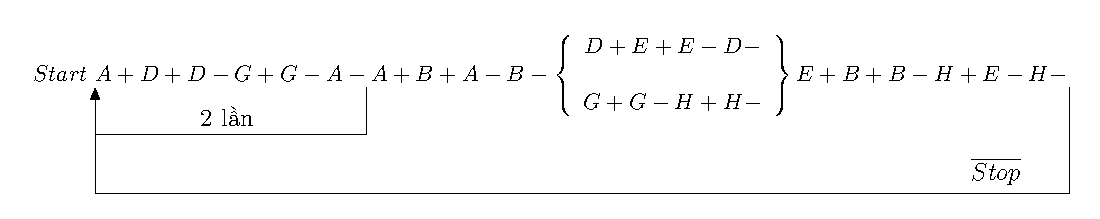
\includegraphics[scale=0.7]{draw-tikz/quatrinh-bt4.pdf}<1->

	\vspace{.5cm}
	\hspace{-1cm}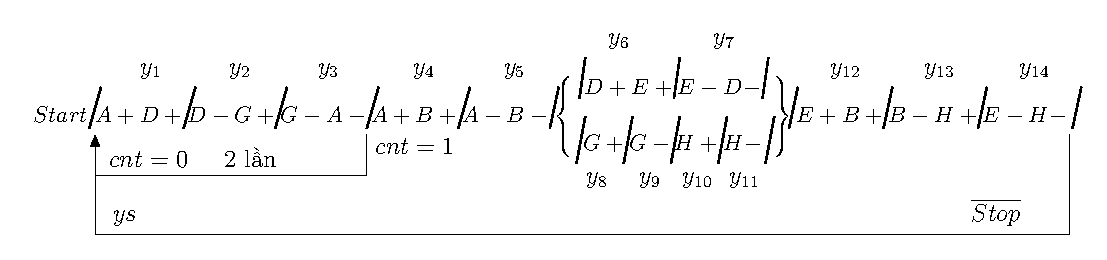
\includegraphics[scale=0.7]{draw-tikz/quatrinh-bt4-buoc1-gomnhom.pdf}<2->
\end{frame}

\subsection*{Viết sơ đồ logic}
\begin{frame}[plain]{Viết sơ đồ logic}
	\vspace{-.5cm}
	\hspace{-1cm}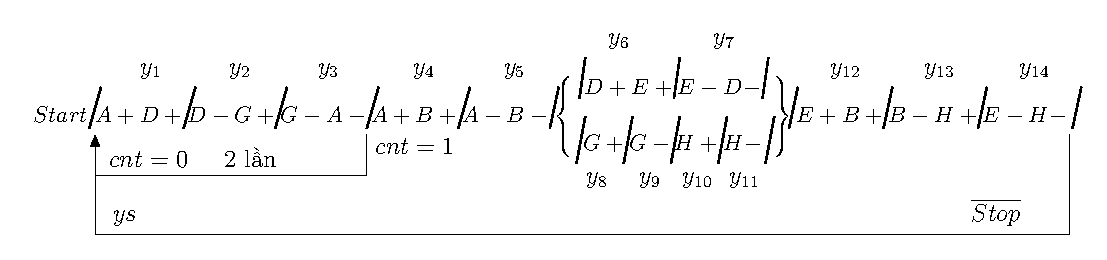
\includegraphics[scale=0.7]{draw-tikz/quatrinh-bt4-buoc1-gomnhom.pdf}\\
	\vspace{-.5cm}
	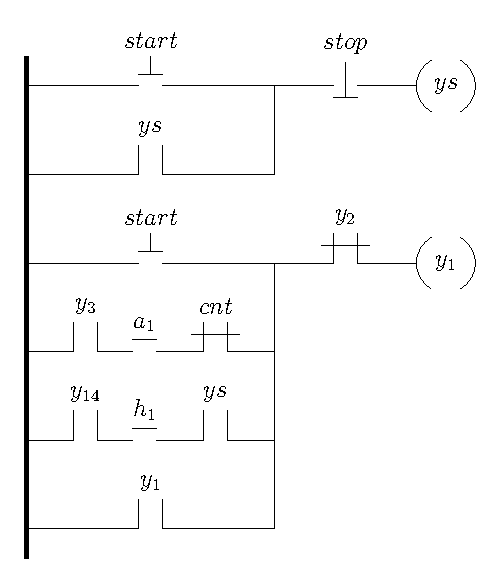
\includegraphics[scale=0.6]{draw-tikz/quatrinh-bt4-buoc2-sodologic-b1.pdf}<1->
	\hspace{0.5cm}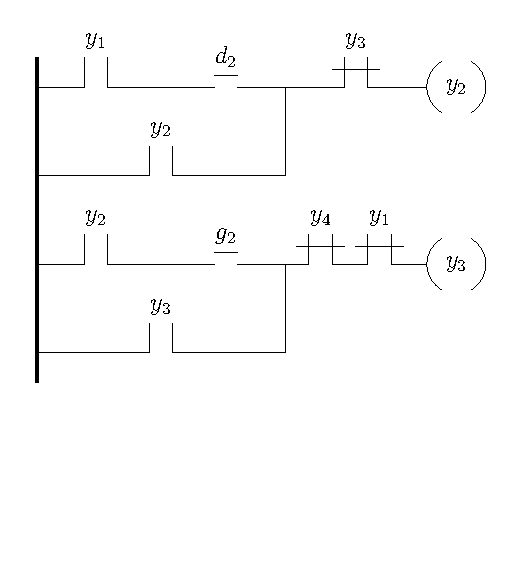
\includegraphics[scale=0.6]{draw-tikz/quatrinh-bt4-buoc2-sodologic-b2.pdf}<2->
\end{frame}

\begin{frame}[plain]{Viết sơ đồ logic}
	\vspace{-.5cm}
	\hspace{-1cm}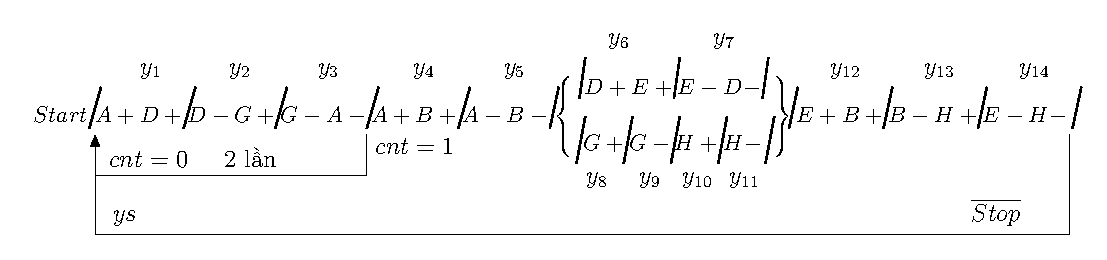
\includegraphics[scale=0.7]{draw-tikz/quatrinh-bt4-buoc1-gomnhom.pdf}\\

	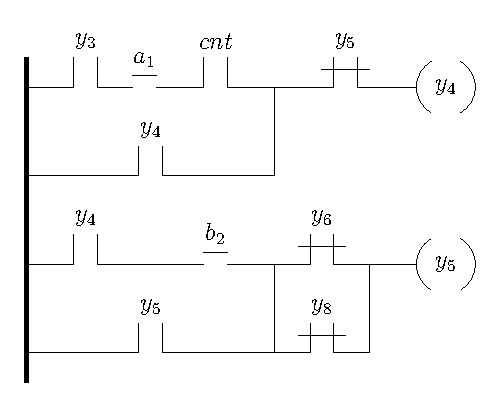
\includegraphics[scale=0.6]{draw-tikz/quatrinh-bt4-buoc2-sodologic-b3.pdf}<1->
	\hspace{0.5cm}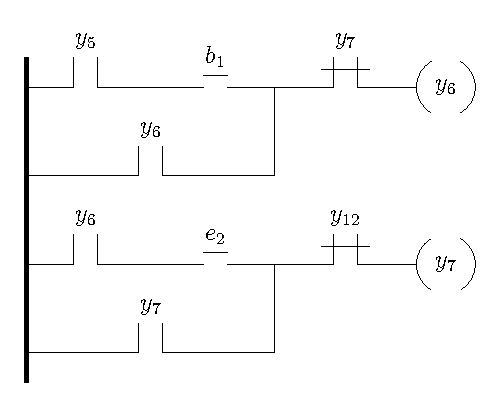
\includegraphics[scale=0.6]{draw-tikz/quatrinh-bt4-buoc2-sodologic-b4.pdf}<2->
\end{frame}

\begin{frame}[plain]{Viết sơ đồ logic}
	\vspace{-.5cm}
	\hspace{-1cm}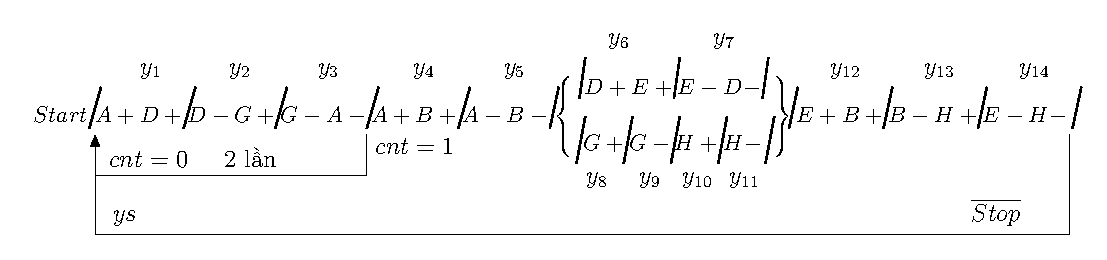
\includegraphics[scale=0.7]{draw-tikz/quatrinh-bt4-buoc1-gomnhom.pdf}\\

	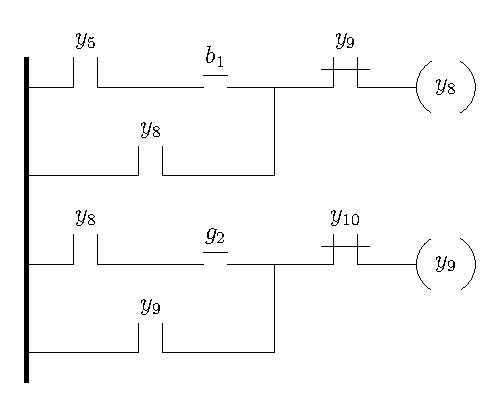
\includegraphics[scale=0.6]{draw-tikz/quatrinh-bt4-buoc2-sodologic-b5.pdf}<1->
	\hspace{0.5cm}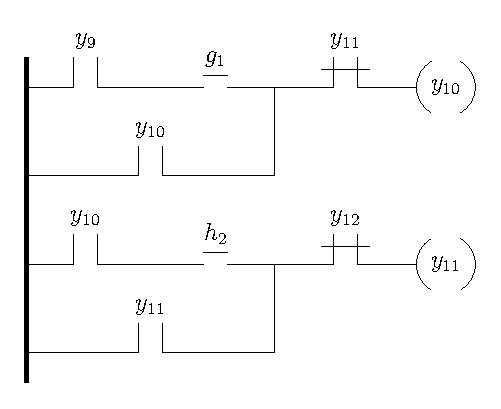
\includegraphics[scale=0.6]{draw-tikz/quatrinh-bt4-buoc2-sodologic-b6.pdf}<2->
\end{frame}

\begin{frame}[plain]{Viết sơ đồ logic}
	\vspace{-.5cm}
	\hspace{-1cm}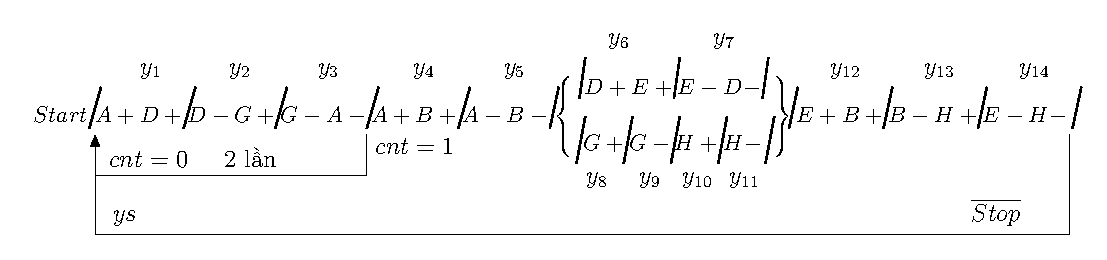
\includegraphics[scale=0.7]{draw-tikz/quatrinh-bt4-buoc1-gomnhom.pdf}\\

	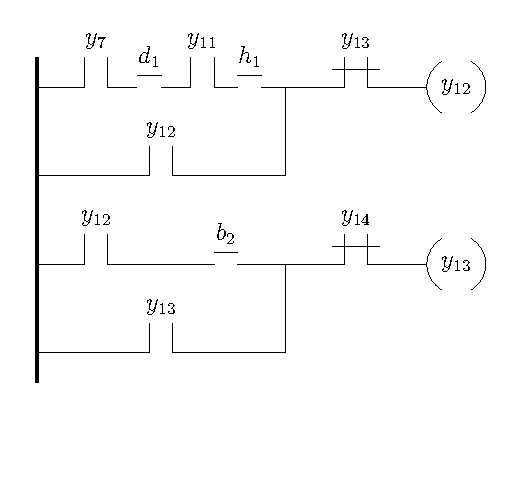
\includegraphics[scale=0.6]{draw-tikz/quatrinh-bt4-buoc2-sodologic-b7.pdf}<1->
	\hspace{0.5cm}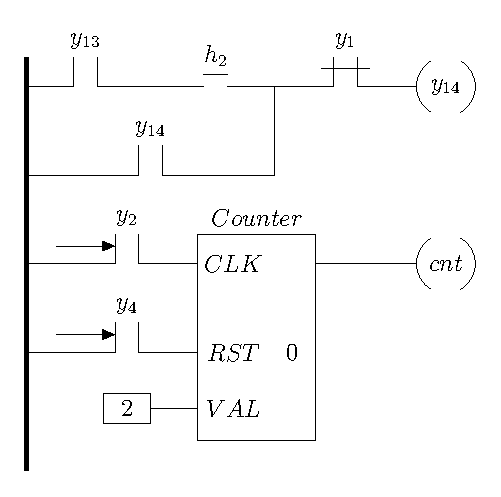
\includegraphics[scale=0.6]{draw-tikz/quatrinh-bt4-buoc2-sodologic-b8.pdf}<2->
\end{frame}

\subsection*{Viết sơ đồ cấp điện}
\begin{frame}[plain]{Viết sơ đồ cấp điện}
		\vspace{-0.5cm}
		\hspace{-1cm}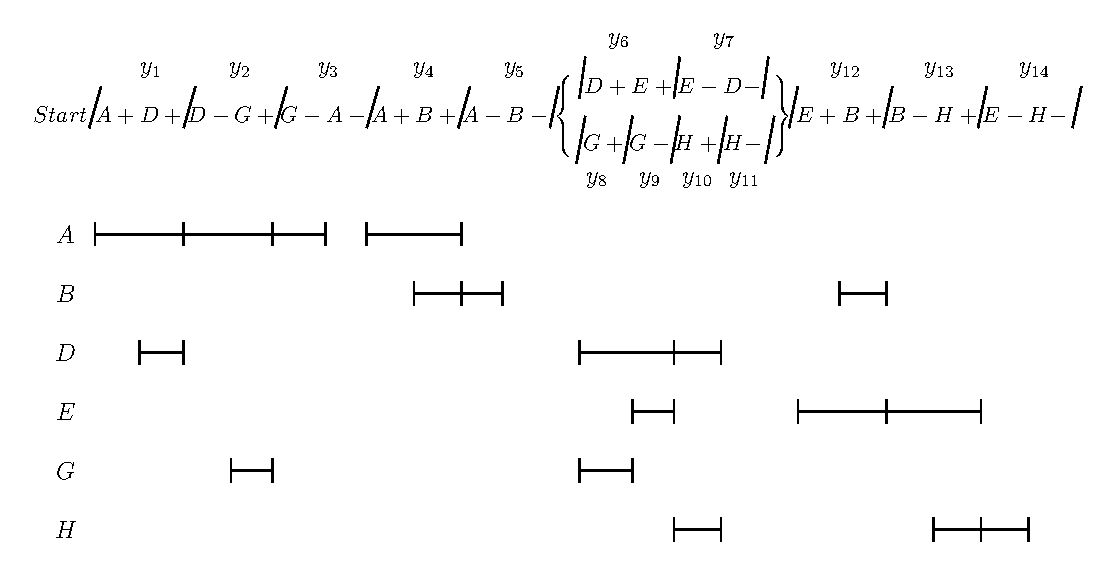
\includegraphics[scale=0.7]{draw-tikz/quatrinh-bt4-buoc3-danhdau.pdf}
\end{frame}

\begin{frame}[plain]{Viết sơ đồ cấp điện}
		\vspace{-0.5cm}
		\hspace{-1cm}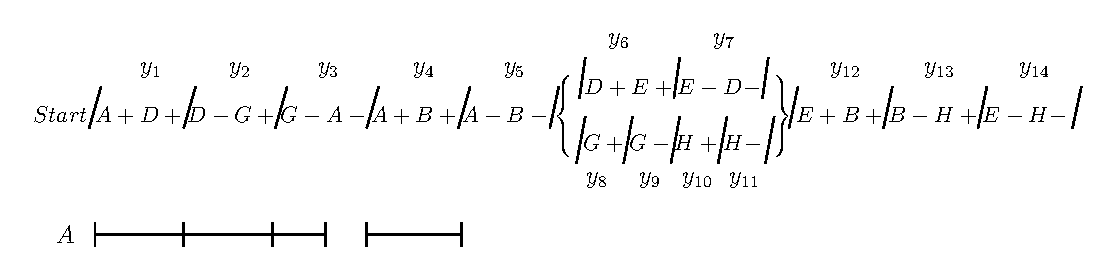
\includegraphics[scale=0.7]{draw-tikz/quatrinh-bt4-buoc3-sodocapdien-A-b1.pdf}\\
		\vspace{-.5cm}
		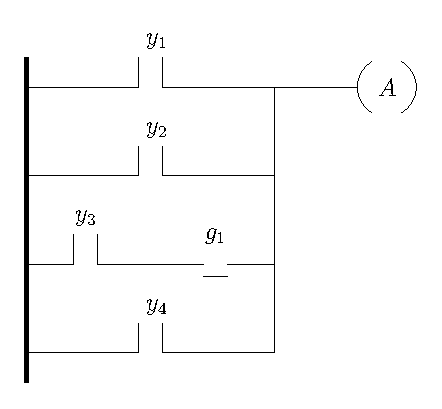
\includegraphics[scale=0.8]{draw-tikz/quatrinh-bt4-buoc3-sodocapdien-A-b2.pdf}
\end{frame}

\begin{frame}[plain]{Viết sơ đồ cấp điện}
		\vspace{-0.5cm}
		\hspace{-1cm}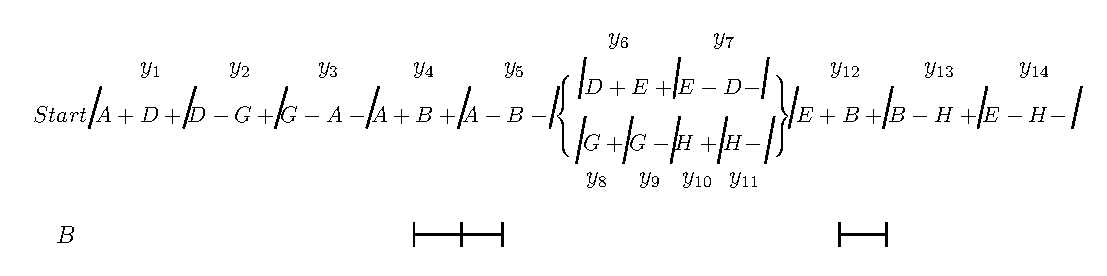
\includegraphics[scale=0.7]{draw-tikz/quatrinh-bt4-buoc3-sodocapdien-B-b1.pdf}\\
		\vspace{-.7cm}
		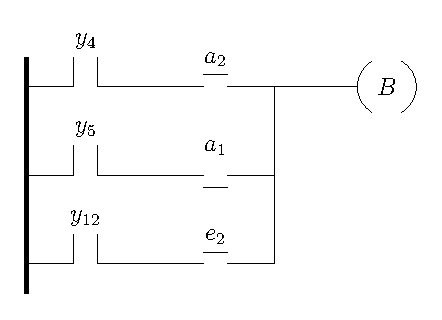
\includegraphics[scale=1.1]{draw-tikz/quatrinh-bt4-buoc3-sodocapdien-B-b2.pdf}
\end{frame}

\begin{frame}[plain]{Viết sơ đồ cấp điện}
		\vspace{-0.5cm}
		\hspace{-1cm}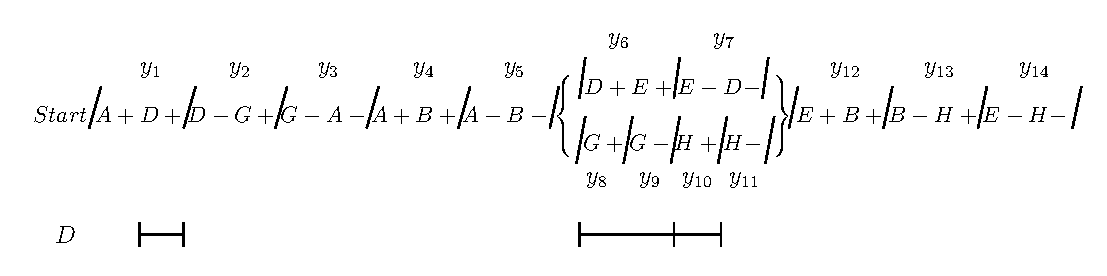
\includegraphics[scale=0.7]{draw-tikz/quatrinh-bt4-buoc3-sodocapdien-D-b1.pdf}\\
		\vspace{-.7cm}
		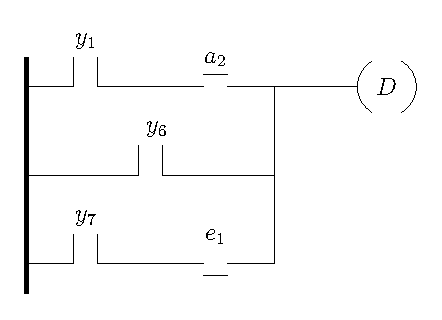
\includegraphics[scale=1.1]{draw-tikz/quatrinh-bt4-buoc3-sodocapdien-D-b2.pdf}
\end{frame}

\begin{frame}[plain]{Viết sơ đồ cấp điện}
		\vspace{-0.5cm}
		\hspace{-1cm}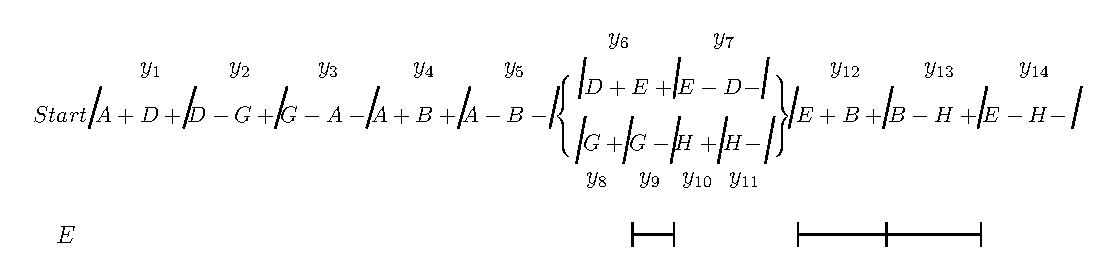
\includegraphics[scale=0.7]{draw-tikz/quatrinh-bt4-buoc3-sodocapdien-E-b1.pdf}\\
		\vspace{-1cm}
		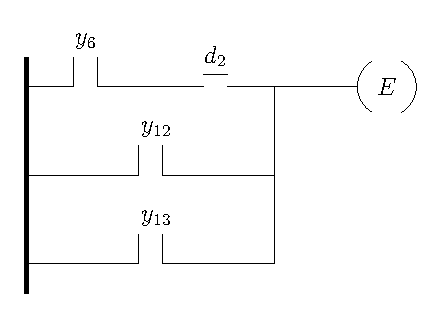
\includegraphics[scale=1.2]{draw-tikz/quatrinh-bt4-buoc3-sodocapdien-E-b2.pdf}
\end{frame}

\begin{frame}[plain]{Viết sơ đồ cấp điện}
		\vspace{-0.5cm}
		\hspace{-1cm}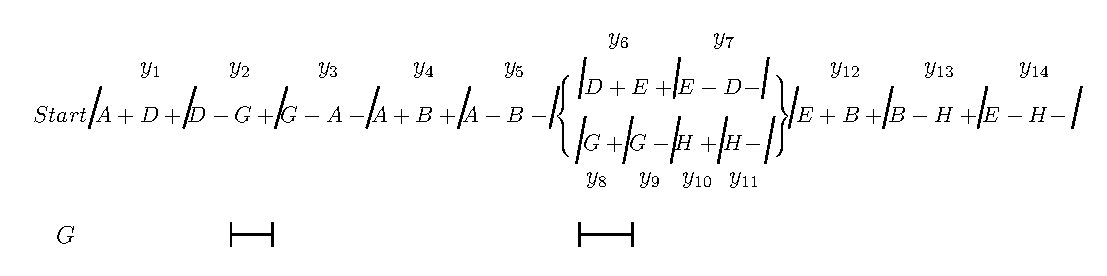
\includegraphics[scale=0.7]{draw-tikz/quatrinh-bt4-buoc3-sodocapdien-G-b1.pdf}\\
		\vspace{-.5cm}
		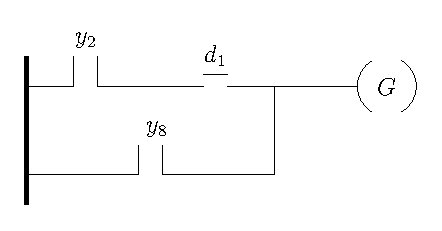
\includegraphics[scale=1.5]{draw-tikz/quatrinh-bt4-buoc3-sodocapdien-G-b2.pdf}
\end{frame}

\begin{frame}[plain]{Viết sơ đồ cấp điện}
		\vspace{-0.5cm}
		\hspace{-1cm}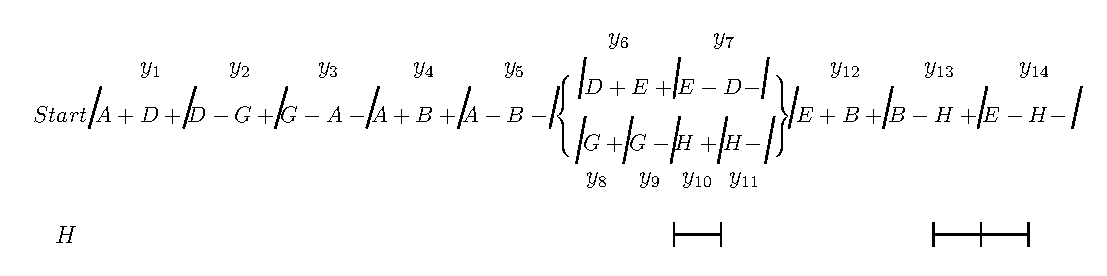
\includegraphics[scale=0.7]{draw-tikz/quatrinh-bt4-buoc3-sodocapdien-H-b1.pdf}\\
		\vspace{-.5cm}
		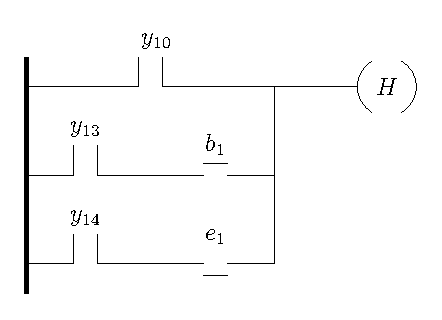
\includegraphics[scale=1]{draw-tikz/quatrinh-bt4-buoc3-sodocapdien-H-b2.pdf}
\end{frame}
\section[Mô phỏng mạch điều khiển]{Mô phỏng mạch điều khiển với Festo Fluidsim và PLC SIM}
\begin{frame}{Mô phỏng sử dụng Festo Fluidsim và PLC SIM}
	\begin{enumerate}
		\justifying
		\item Theo cách sơ đồ nối điện.
		
		\item Theo ngôn ngữ Leader.
		
		\item Lập trình trên phần mềm PLC.
	\end{enumerate}
\end{frame}
%--------------------------------------------------------------------------------
%--------------------------------------------------------------------------------
% Tai lieu tham khao
\section*{Tài liệu tham khảo}
\begin{frame}{Tài liệu tham khảo}
\begin{footnotesize}
\begin{enumerate}[{[1].}]
\justifying
\item \href{https://www.youtube.com/watch?v=VbrZZ7Jg09U&list=PLkemUmoYKlGwmuG1mLVB_VnRhW-h57giK}{Thủy lực -- Khí nén}, Đỗ Đức Khánh, Youtube, Ngày 04 tháng 03 năm 2016.

\item \href{https://www.art-systems.de/fluidsim/download/v4/hb-eng-h4.pdf}{FESTO FluidSIM$^\circledR$ 4 Hydraulics -- User’s Guide}, Art Systems, 
Edition 08/2007.

\item \href{https://www.researchgate.net/publication/278154968_Design_and_Simulation_of_Electro-Pneumatic_Motion_Sequence_Control_Using_FluidSim}{Design and Simulation of Electro-Pneumatic Motion Sequence Control Using FluidSim}, Ravi Kumar -- Jay Robert Del Rosario, January 2014.
\end{enumerate}
\end{footnotesize}
\end{frame}
%--------------------------------------------------------------------------------
%--------------------------------------------------------------------------------
% Lời cảm ơn
\section*{Lời cảm ơn}
\begin{frame}
\justifying
\large \alert{Cảm ơn Thầy và các bạn đã quan tâm theo dõi phần trình bày của nhóm!}
\end{frame}
\end{document}